\documentclass[a4paper, 11pt]{scrartcl}
\usepackage{a4}


\usepackage[utf8]{inputenc}
\usepackage{dsfont}
\usepackage{amsmath}
\usepackage{graphicx}
\usepackage{here}
\usepackage[section]{placeins}
\usepackage[ngerman]{babel}
\usepackage{caption}
\usepackage{subcaption}
\usepackage[colorlinks, pdfpagelabels, pdfstartview = FitH, bookmarksopen = true, bookmarksnumbered = true, linkcolor = black, plainpages = false, hypertexnames = false, citecolor = black] {hyperref}

\parindent 0pt	


\title{Dokumentation der Projektarbeit}
\author{Florian Weber - 44907}
\date{\today}

\begin{document}
\maketitle	%Deckblatt
\newpage

\tableofcontents 	%Inhaltsverzeichnis
\listoffigures		%Bildverzeichnis
\newpage

\section{Einleitung}
\subsection{Zielsetzung}
\newpage

\section{Funktion}
	Im Folgenden wird der grundlegende Aufbau der Carrera Bahn erklärt.

	Diese Beschreibung ist immer nur für Bahn-A, da die 
	Bahn-B analog dazu funktioniert. Dazu wird immer wieder auf die Abbildung \ref{img:signalfluss}, sowie auf die \\Abbildung 
	\ref{img:carrerakomplett} Bezug genommen.
	\begin{figure}[h]
		\centering
		\includegraphics[width=0.85\textwidth]{bilder/signalfluss.pdf}
		\caption{Signalfluss}
		\label{img:signalfluss}
	\end{figure}
	\begin{figure}[h]
	\centering
	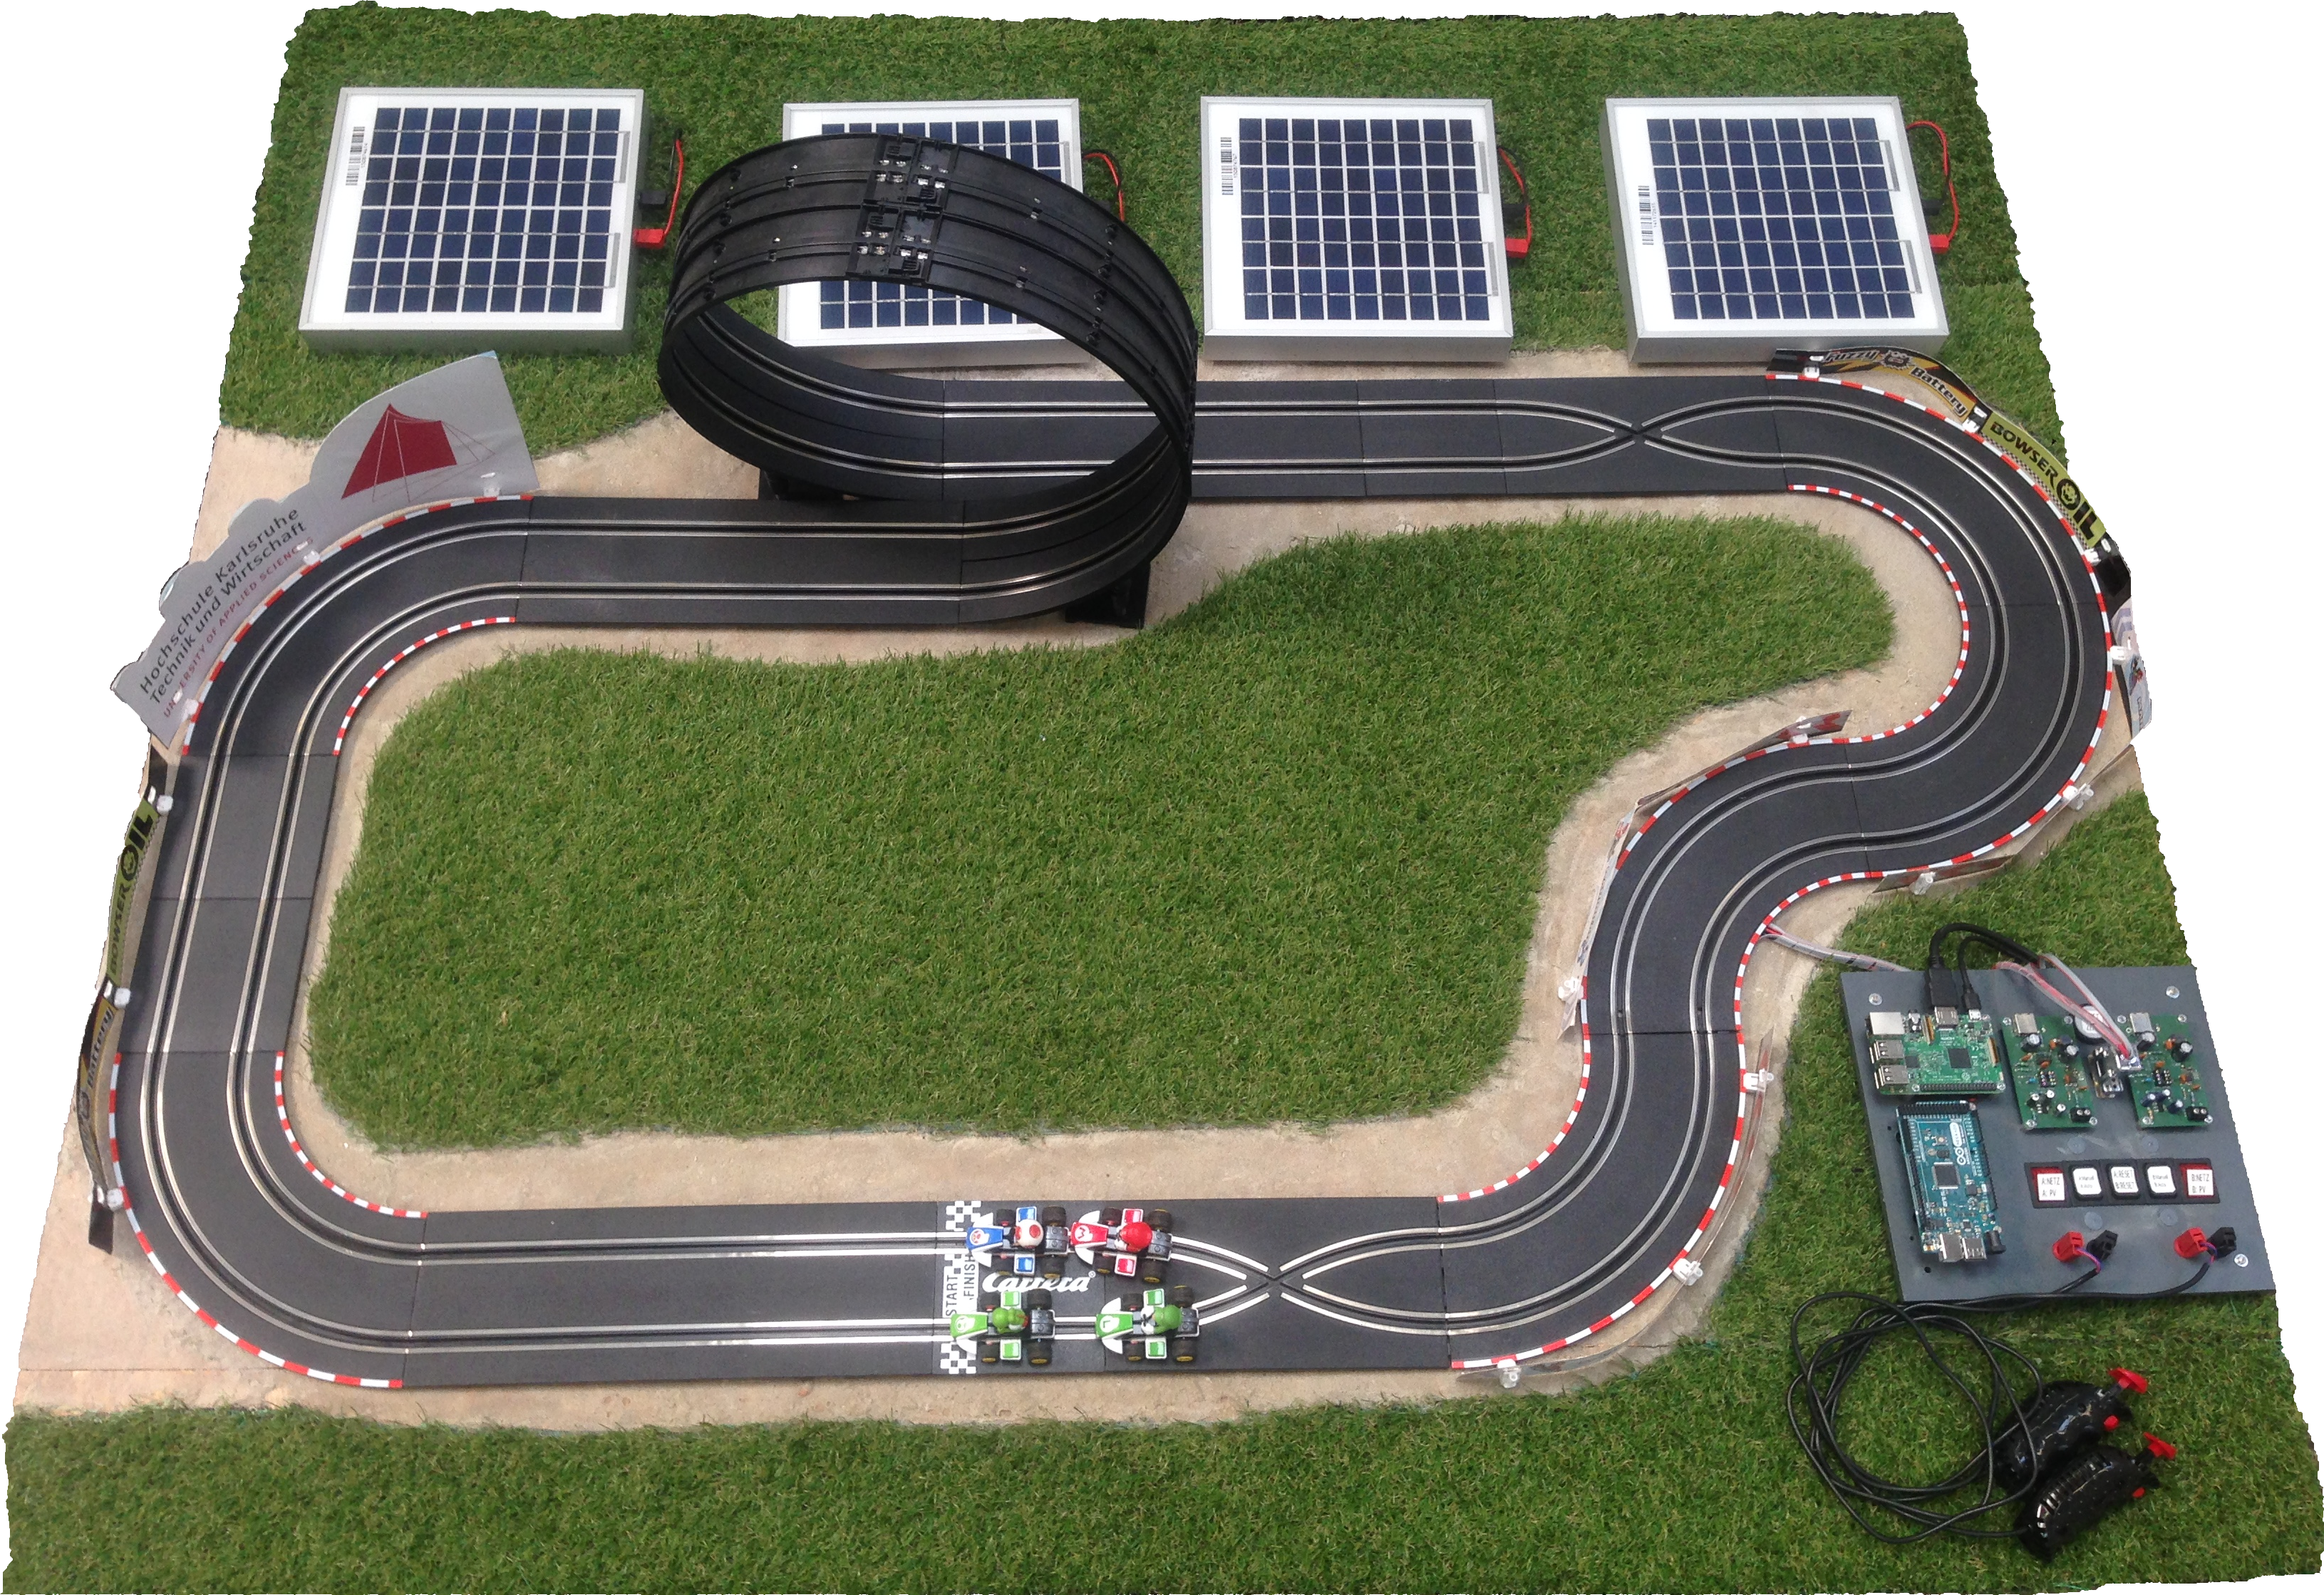
\includegraphics[width=0.85\textwidth]{bilder/Carrerabahnroh.png}
	\caption{Überblick über die Carrera-Bahn}
	\label{img:carrerakomplett}
	\end{figure}
	\newpage

	\subsection{Sensoren}
		Pro Schiene gibt es 3 Sensoren die als Gabellichtschranke ausgeführt sind. Sensor 0 befindet sich am Start, Sensor 1 vor dem Looping und 		Sensor 2 Nach dem Looping.\\

		Sensor 0 wird im Wesentlichen nur zur Zeitmessung genutzt, dazu später mehr.
		Sensor 1 wird genutzt um ein Signal zu generieren, so dass die Steuerung das Auto im Automatik-Modus für den Looping beschleunigen kann. 		Das Signal von Sensor 2 wird schließlich genutzt um nach dem Looping wieder die langsame Geschwindigkeit zu triggern.\\
		Im manuellen Modus dienen die Sensoren nur zur Zeitmessung für die Visualisierung.
		Da die Flanke nur sehr kurz ist, lässt sich diese nicht per Polling ohne Aliasing Effekte digitalisieren. Stattdessen wurden die Hardware 		Pin Change Interrupts des Atmega2560 genutzt.
	\subsection{Bedienschnittstelle}
		\begin{figure}[h]
			\centering
			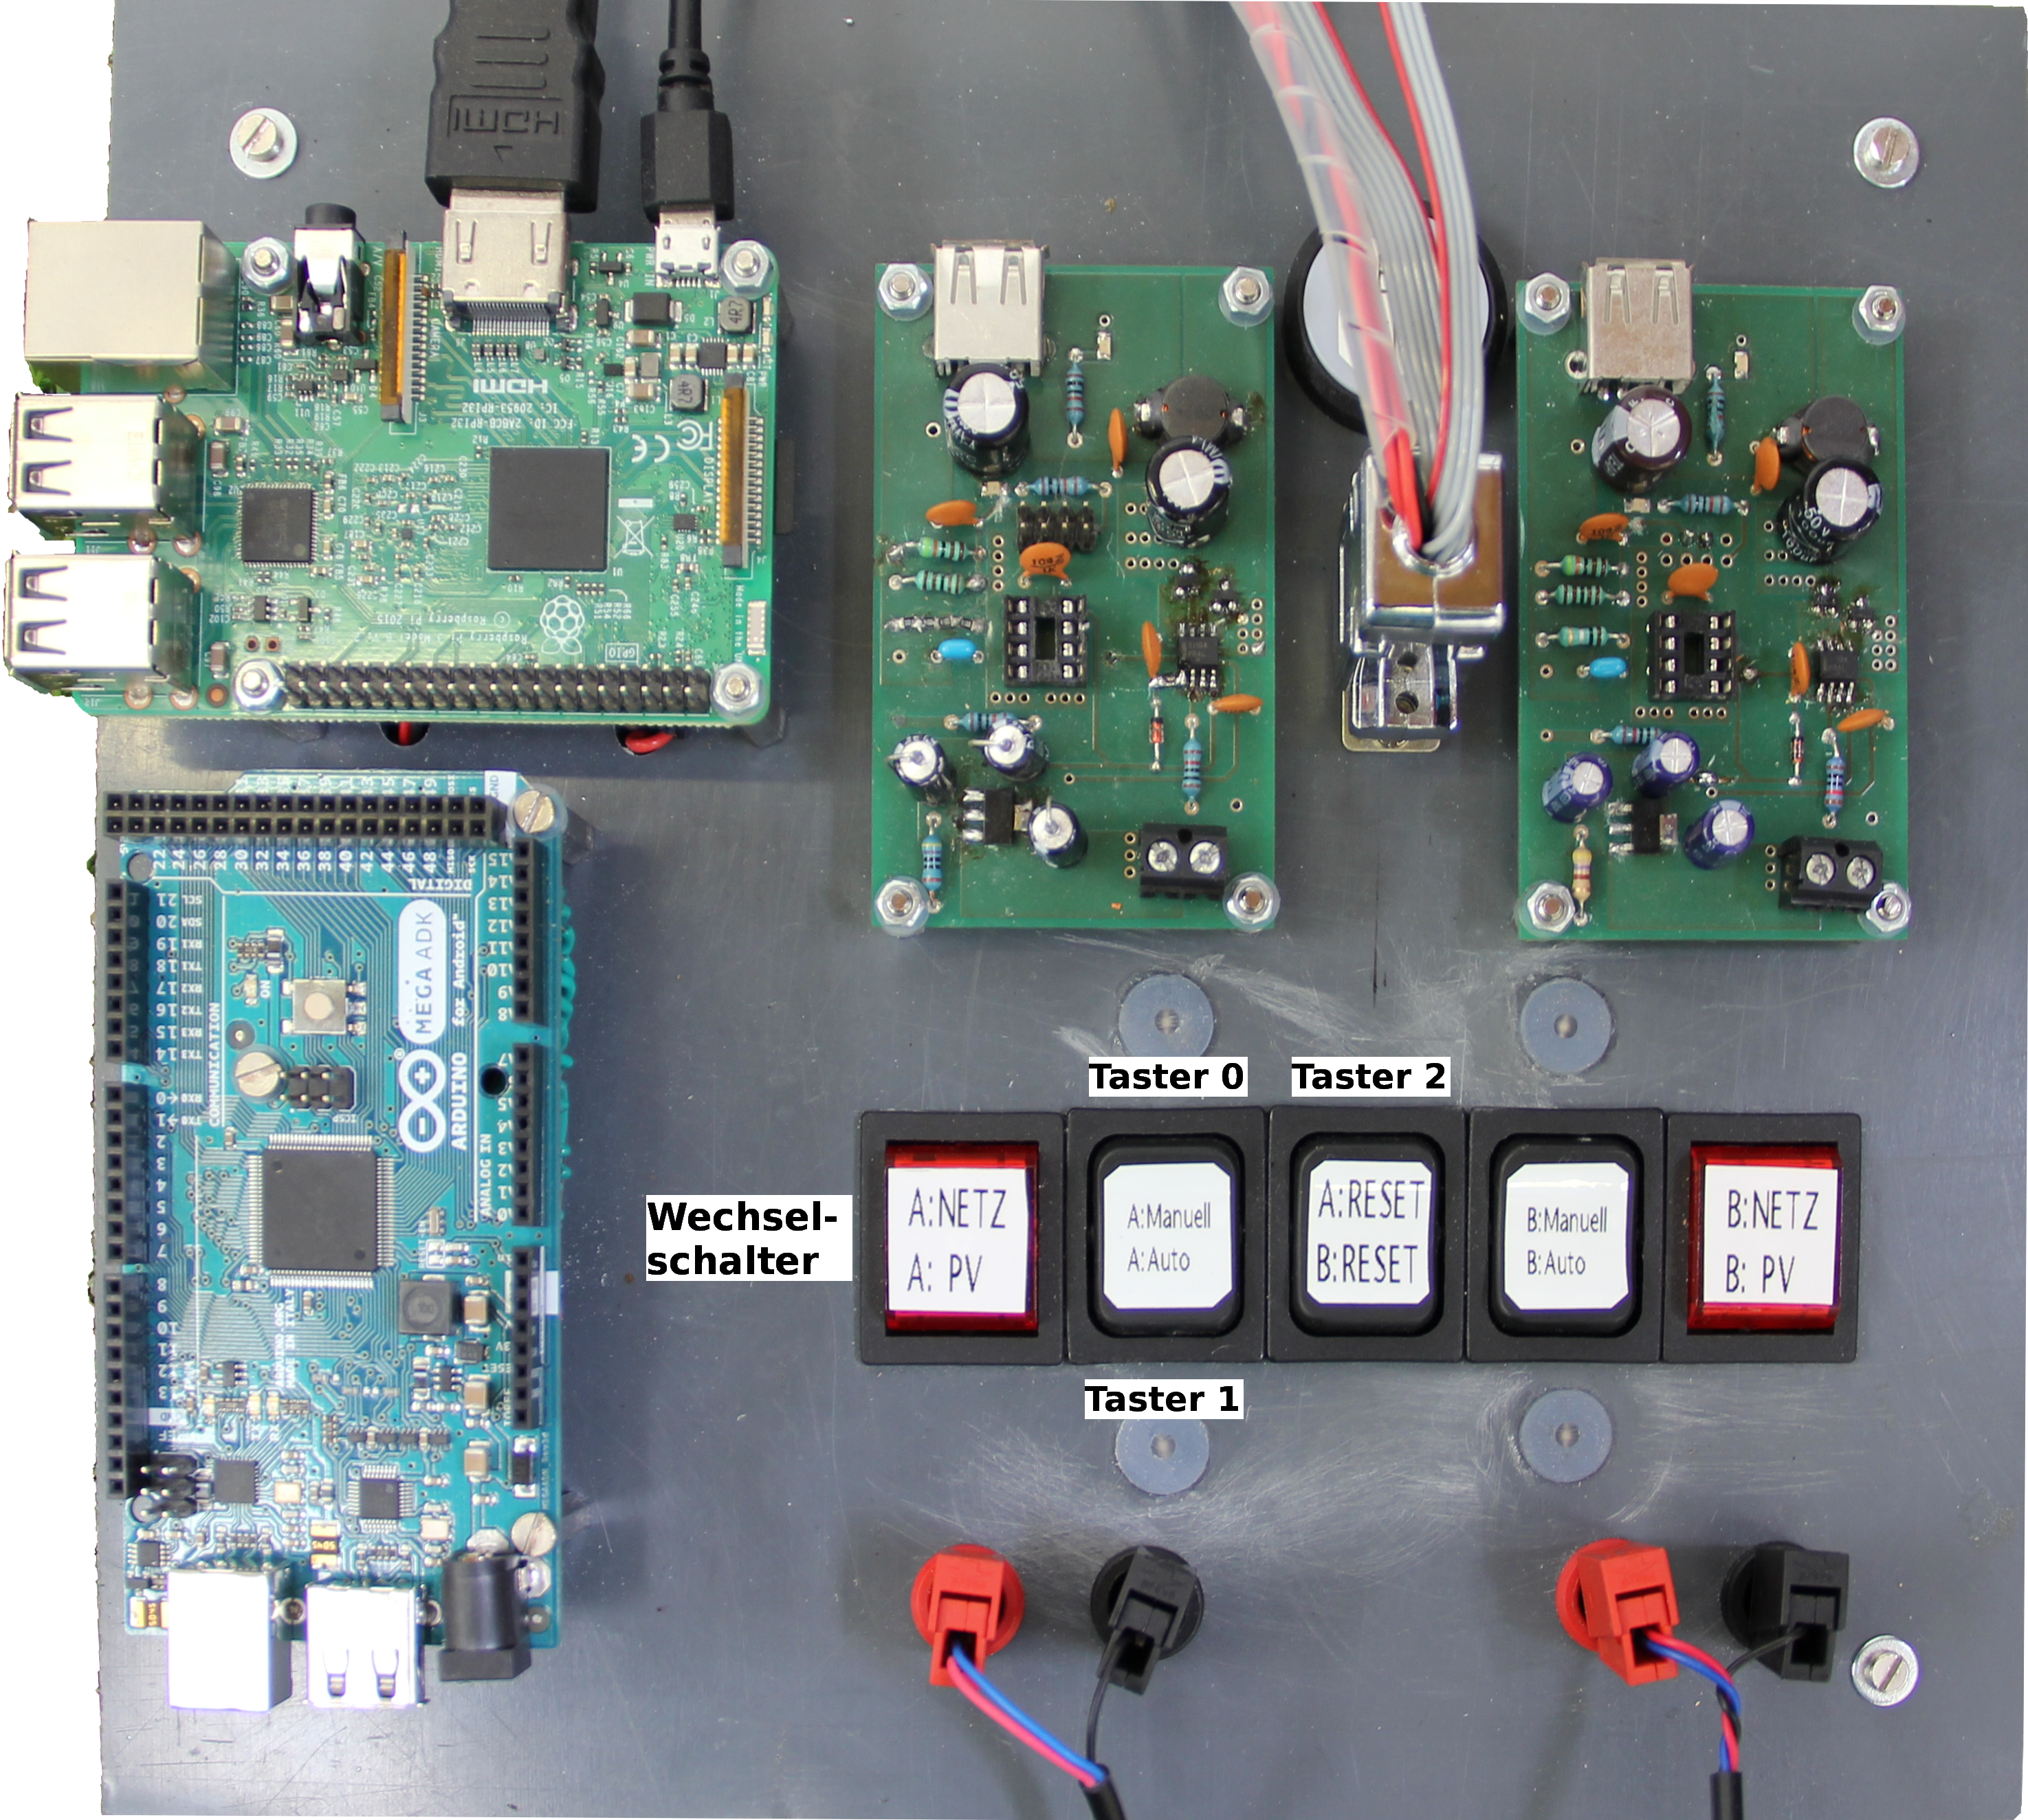
\includegraphics[width=0.85\textwidth]{bilder/hid.png}
			\caption{Bedienschnittstelle}
			\label{img:hid}
		\end{figure}
		Das HID besteht aus 3 Tastern und einem Wechselschalter mit Mittelstellung je Bahn.
		Der Wechselschalter ist zum Auswählen, ob die Bahn mit Energie aus den Solarpanels betrieben wird, oder mit Netzstrom. Ist Dieser in Mittelstellung, wird die Bahn nicht versorgt und das Auto steht - unabhängig des gewählten Modus.
		Über Taster 0 beziehungsweise Taster 1 lässt sich der Modus der Bahn auswählen, welcher durch die LEDs bei den Tastern signalisiert wird. \\Hier steht Automatik und Manuell zur Auswahl.
		Mit Taster 2 lässt sich der Regler der Bahngeschwindigkeit genauer -  Spannung außerhalb des Loopings, auf seinen Startwert zurücksetzen.
	\subsection{Arduino}
		Beim Arduino handelt es sich um einen einfachen Arduino Mega 2560 ADK.\\
		Dieser wurde gewählt da es sich um eine preiswerte Platine handelt, die bereits die wichtigsten Beschaltungen des Mikrocontroller enthält wie zum beispiel die Abblockcondensatoren an der Versorgungsspannung aber auch einen USB-Seriell Wandler den man nutzen kann um sich Daten parallel zum Prozess an ein Terminal auszugeben.
		Letzteres lässt sich sehr gut für das Debugging nutzen.
	\subsection{RaspberryPi}
		Die Visualisierung ist durch ein RaspberryPi Model 3 B realisiert. Dieser empfängt per Uart die codierten Signale der Sensoren, sowie des Reset Tasters der Visualisierung.
		Die Visualisierung war zu Beginn der Projektarbeit bereits vorhanden und in Form eines Python Skripts implementiert.
	\subsection{Tiefsetzsteller}
		Die Tiefsetzsteller fungieren als Stellglieder der Spannungsregelungen der Bahnen. Jeder bekommt sein PWM-Signal(Steuergröße) direkt vom Arduino. Desweiteren ist über ein Shunt eine Strommessung realisiert. Der Wert liegt zwar im Arduino digital vor, wird allerdings nicht weiter verarbeitet und ist lediglich für weiterführende Projekte gedacht. Da die Ausgangsspannung des Tiefsetzsteller größer sein kann wie die Referenzspannung des ADC, wird diese über einen Spannungsteiler angepasst und auf einen Kanal des ADC geführt. Diese Spannung stellt eine Regelgröße dar.
	\newpage
	\subsection{Software}
		\subsubsection{RaspberryPi}
			Bei der Software die auf dem RaspberryPi ausgeführt wird, handelt es sich um ein Python Skript. Dieses war zu Beginn der Projektarbeit bereits vorhanden und hat die Sensoren der Bahn parallel eingelesen. Mit den Flanken der Sensoren wurde die Rundenzeit gemessen und die Bestzeit ermittelt.\\
			Dieses Skript wurde größtenteils übernommen und lediglich in der Richtung abgeändert, dass die Trigger-Signale der Sensoren nun über die Serielle Schnittstelle dem Pi mitgeteilt wurden. Des Weiteren wurden diverse Bugs behoben wie zum Beispiel die zu geringe Framerate der Visualisierung. Als serielle Schnittstelle wurde "ttyAMA0" benutzt.
		\newpage	
		\subsubsection{Arduino}
			Die Software des Arduino wurde, wie oben bereits erwähnt, nicht in der Arduino Entwicklungsumgebung geschrieben. Stattdessen habe ich auf die IDE "AtmelStudio6" zurückgegriffen und den Mikrocontroller per ISP beschrieben. Der Bootloader des Arduino musste dazu entfernt werden.
			Gründe dazu waren unter anderem die Wahl der Sprache C++, aber auf die Möglichkeit direkt auf die Hardware zuzugreifen(Timer, Hardwareinterrupts...). Letzteres ist notwendig um das Timing des Controllers exakt zu steuern.\\
			
			
			\begin{figure}[h]	
				\centering
				\begin{subfigure}{0.47\textwidth}
					\centering
					\includegraphics[width=1.1\textwidth]{bilder/Interrupt_Programme.png}
					\caption{Interruptgesteuerter \\Programmablauf}
					\label{InterruptgesteuerterProgrammablauf}		
				\end{subfigure}
				\begin{subfigure}{0.47\textwidth}
					\centering
					\includegraphics[width=0.55\textwidth]{bilder/Sequentielle_Programme.png}
					\caption{Sequentieller \\Programmablauf}
					\label{SequentiellerProgrammablauf}
				\end{subfigure}
				\caption[Möglichkeiten zum Programmablauf]{Möglichkeiten zum Programmablauf\\Quelle:Mikrocontroller.net}\label{Programmablauf}
			\end{figure}
			Der Programmablauf ist größtenteils Interruptgesteuert.
			Dies hat den Vorteil, dass das Timing nicht mehr von der Länge der MainLoop abhängt und Dinge wie zum  Beispiel der Regelalgorithmus immer in der selben Frequenz ausgeführt werden.
					
	\newpage
	
\section{Bedienungsanleitung}
Die CarreraBahn besitz 2 auswählbare Modi. Den Modus "Manuelles Fahren", sowie den Modus "Automatisiertes Fahren".
\subsection{Manuelles Fahren}

\subsection{Automatisiertes Fahren}
\newpage

\section{Zusammenfassung}
\newpage

\section{Quellenverzeichnis}
\newpage

\section{Anhang}
\subsection{Pinbelegung}
\subsubsection{Arduino}
\subsubsection{RaspberryPi}
\end{document}
